\section{MPI Point-to-Point Communication}
\subsection{Required submission files}
\begin{enumerate}
	\item \hl{The updated \emph{gauss.c} file.}

		\verb!Data/MPI_P2P/gauss.c!

	\item \hl{The new performance plots and description in the report.}

		Please refer to Fig. \ref{fig:compute_multdomain_nb_baseline}, \ref{fig:compute_multproc_nb_baseline}, \ref{fig:mpi_multdomain_nb_baseline}, \ref{fig:mpi_multproc_nb_baseline}, \ref{fig:total_multdomain_nb_baseline}, and \ref{fig:total_multproc_nb_baseline}.

\end{enumerate}

\subsection{Questions}
\begin{enumerate}
	\item \hl{Which non-blocking operations were used? Justify your choice.}

	As this assignment was about point-to-point (P2P) communication, we restricted the choice of possible communication methods just to the P2P ones, avoiding collectives.

	The non-blocking P2P communication methods used are \verb!MPI_Isend()! and \verb!MPI_Irecv()!.

	\verb!MPI_Isend()! was used to avoid any waiting time on the sender in case the receiver has not reached the communication step yet. In this code the local computation can always proceed independently of the data being received on other processes and there is no risk of overwriting the send buffer.

	\verb!MPI_Irecv()! was instead used to try to anticipate the communication, e.g. by calling it during a previous loop iteration with respect to when the data is actually required.

	Not all the original blocking P2P communication calls were translated into their non-blocking counterparts: for example some \verb!MPI_Recv()! calls during the initial data distribution phase have been kept in their blocking version as there was no benefit in using the non-blocking version, i.e. no possibility to overlap the communication with any computation task.

	\item \hl{Was communication and computation overlap achieved? Use Vampir.}

	Not really. It is true that some degree of overlap whas achieved mainly by performing the communication for the following loop iteration while computing the current one. However the Vampir output \todo{Here refer to Vampir screenshot} confirms the theoretical understading of the gaussian elimination as an inherently sequential algorithm. In the figure \todo{ref} we often see red patches within the green bands: these are because processes are waiting for information from the ones with lower rank in order to perform their calculations.

	We also changed the communication pattern so that pivots are propagated after each row computation, instead of communicating after the computation entire local block. This has the benefit of allowing an earlier start of all the processes, however it does not really improve the cumulative time spent by the various processes waiting for data.

	So there is some overlap, but the inherent load imbalance of the algorithm and the sequential dependencies across the processes basically nullify any benefit coming from the computation-communication overlap.

	\item \hl{Was a speedup observed versus the baseline for the Sandy Bridge and Haswell nodes?}

	On average, the non-blocking version performed slightly better than the baseline, however it does not constitute a significant speedup by any means.\todo{Here refer to NB vs Baseline total time plot (or compute time one)}

	This is, again, due to the inherently unbalanced nature of Gaussian Elimination: each process needs the data computed by the previous ones and the further it proceeds in the computation, the more processes are left idle.
	
	
	    	\begin{figure}[h] % h=here, t=top, b=bottom, p=(extra)page, !=force
		\hspace*{-0.25\linewidth}\begin{tabular}{cc}
			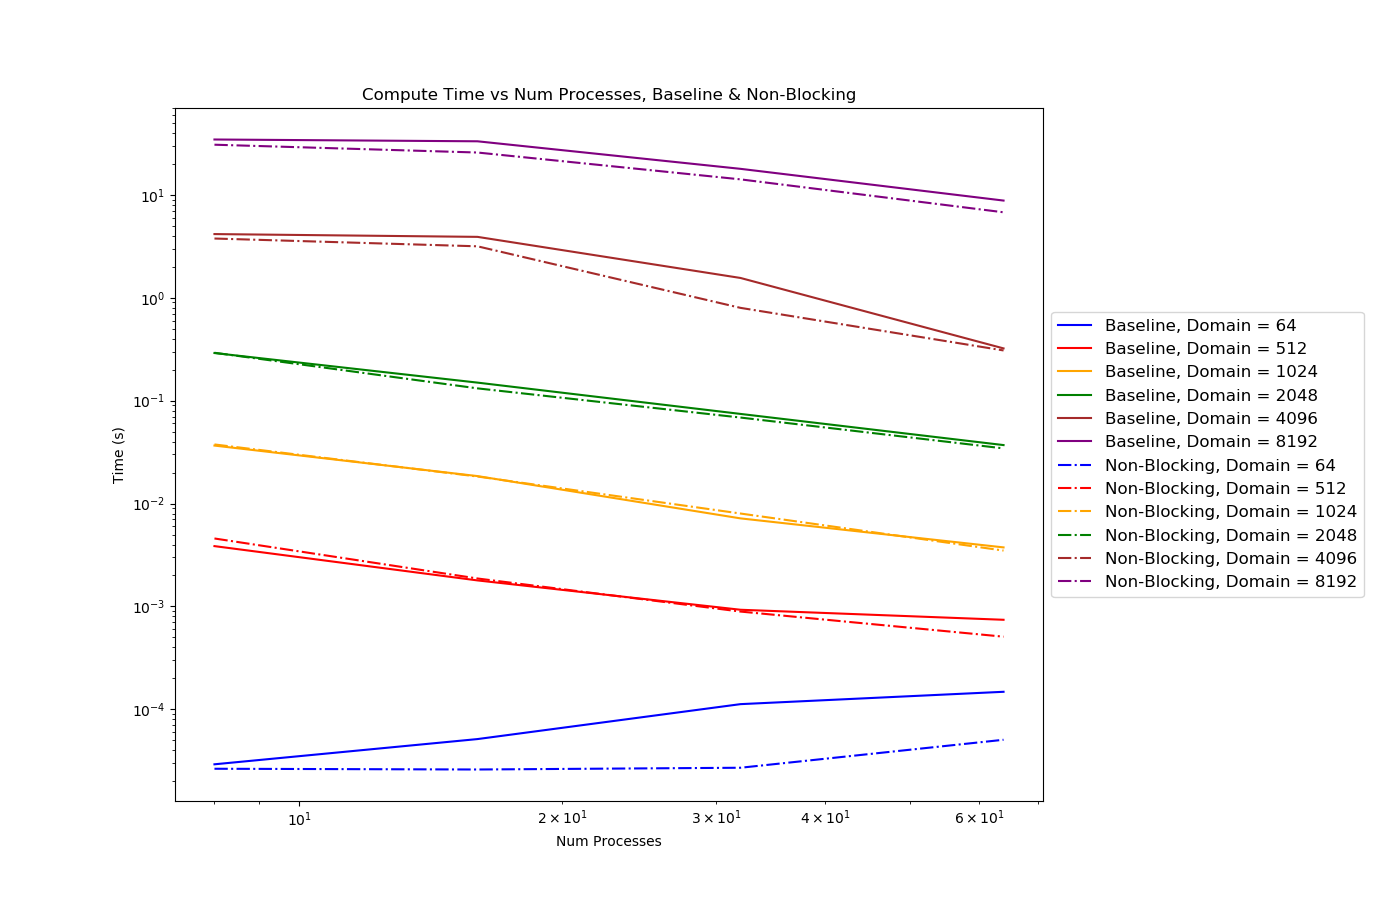
\includegraphics[width=.75\linewidth]{MPI_p2p/compute_multdomain_haswell_nb_baseline.png} & 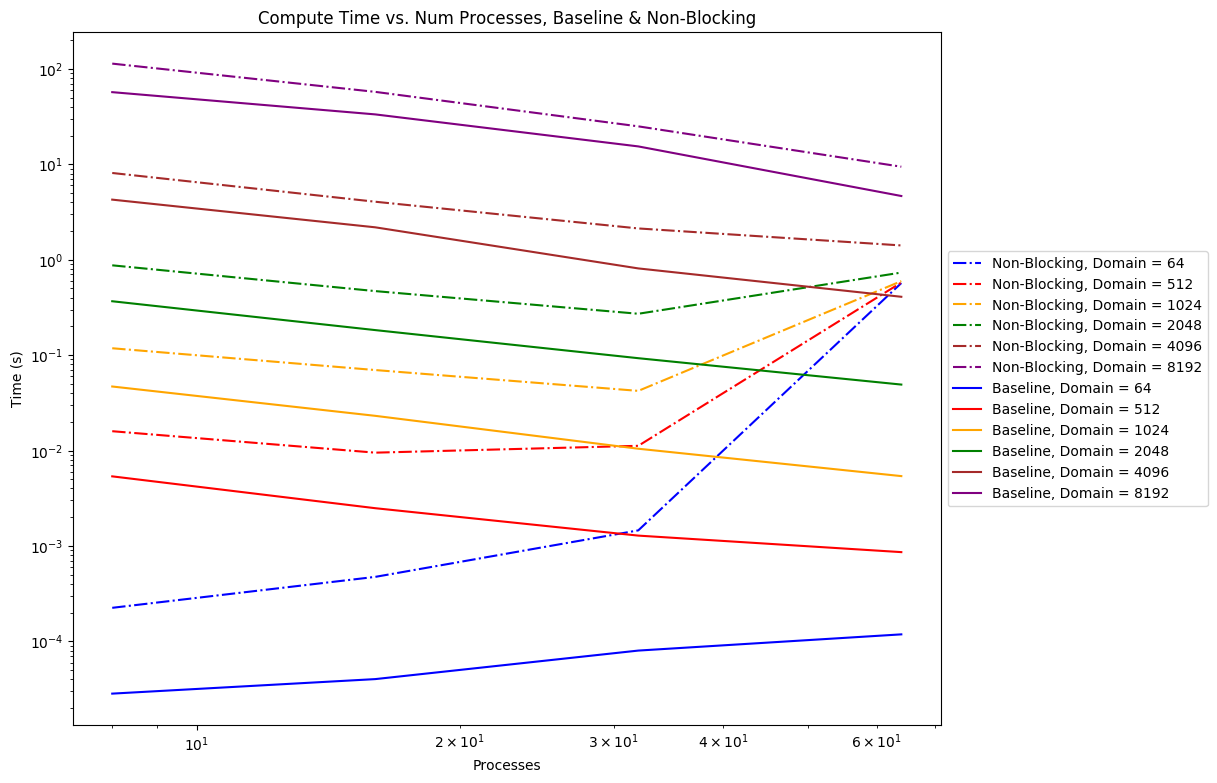
\includegraphics[width=.75\linewidth]{MPI_p2p/compute_multdomain_sandy_nb_baseline.png} \\
			(a) Haswell &  (b) Sandy Bridge\\[6pt]
		\end{tabular}
		\caption{Compute Time vs. \#Processes., Non-Blocking vs. Baseline}
		\label{fig:compute_multdomain_nb_baseline}
	\end{figure}
	
	\begin{figure}[h] % h=here, t=top, b=bottom, p=(extra)page, !=force
		\hspace*{-0.25\linewidth}\begin{tabular}{cc}
			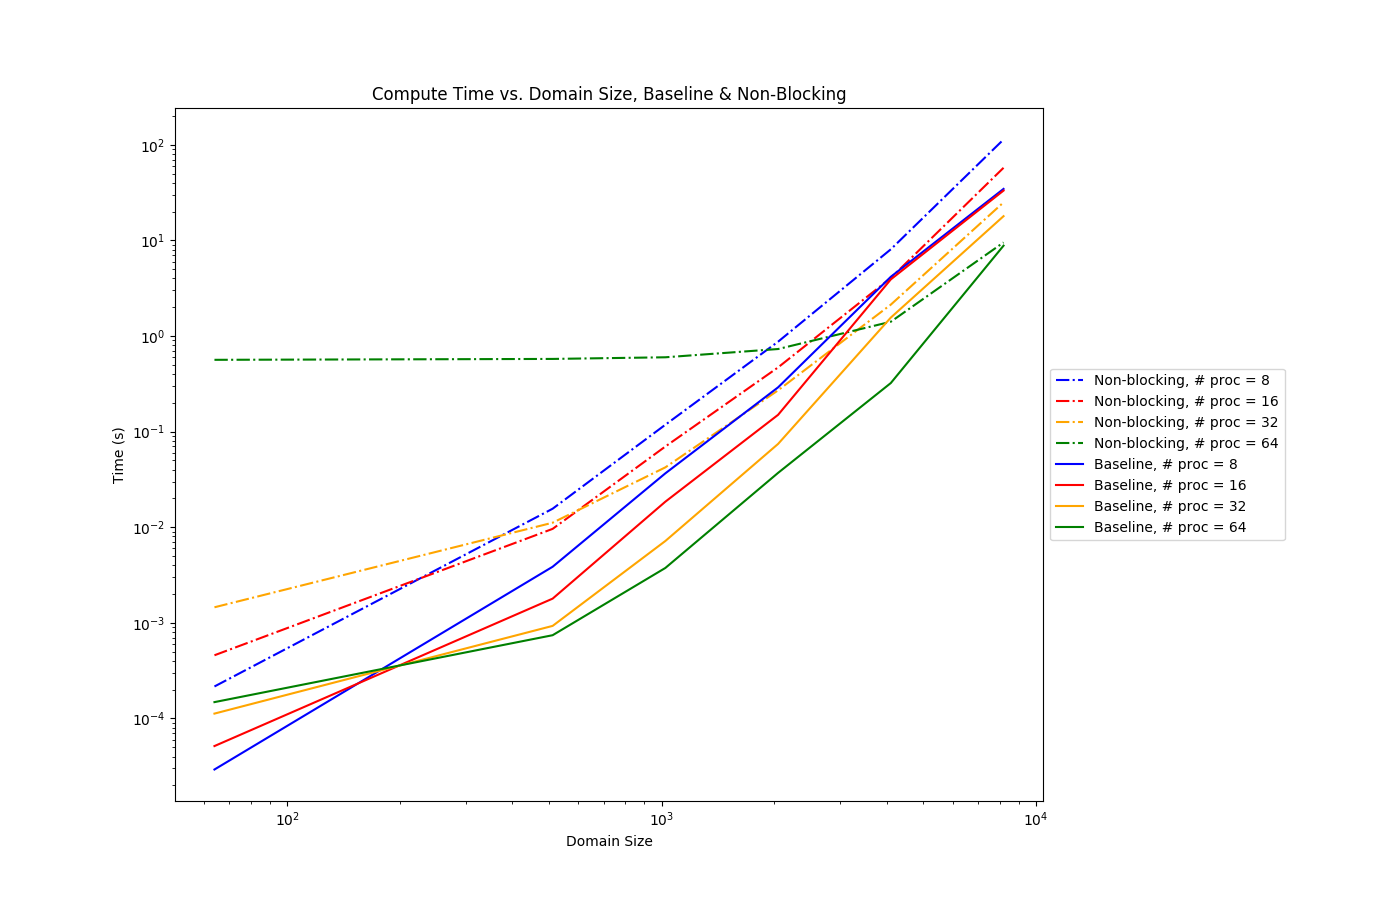
\includegraphics[width=.8\linewidth]{MPI_p2p/compute_multproc_haswell_nb_baseline.png} & 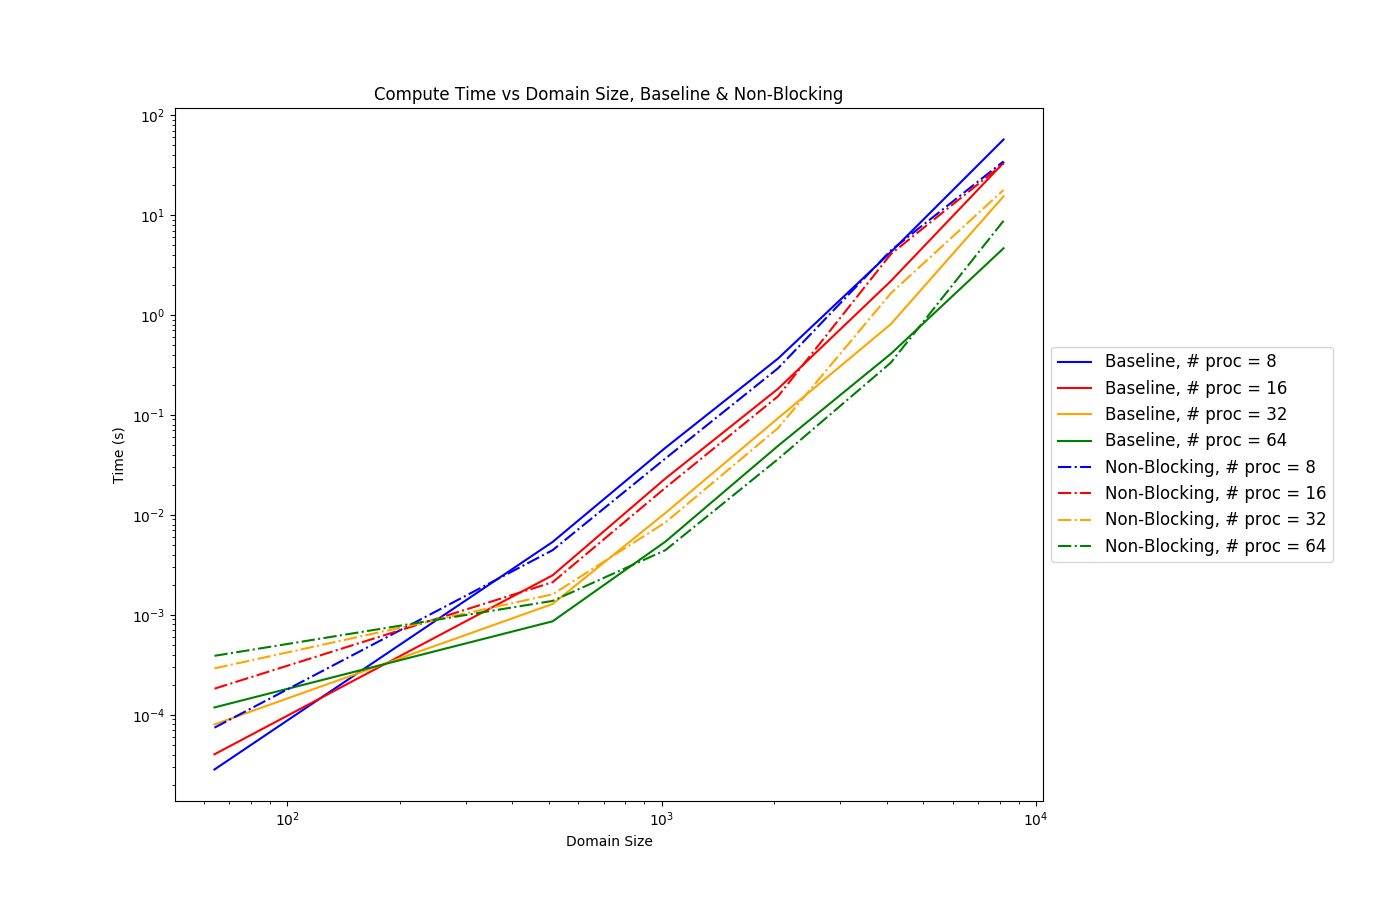
\includegraphics[width=.8\linewidth]{MPI_p2p/compute_multproc_sandy_nb_baseline.png} \\
			(a) Haswell &  (b) Sandy Bridge\\[6pt]
		\end{tabular}
		\caption{Compute Time vs. Domain Size., Non-Blocking vs. Baseline}
		\label{fig:compute_multproc_nb_baseline}
	\end{figure}
	
		\begin{figure}[h] % h=here, t=top, b=bottom, p=(extra)page, !=force
		\hspace*{-0.25\linewidth}\begin{tabular}{cc}
			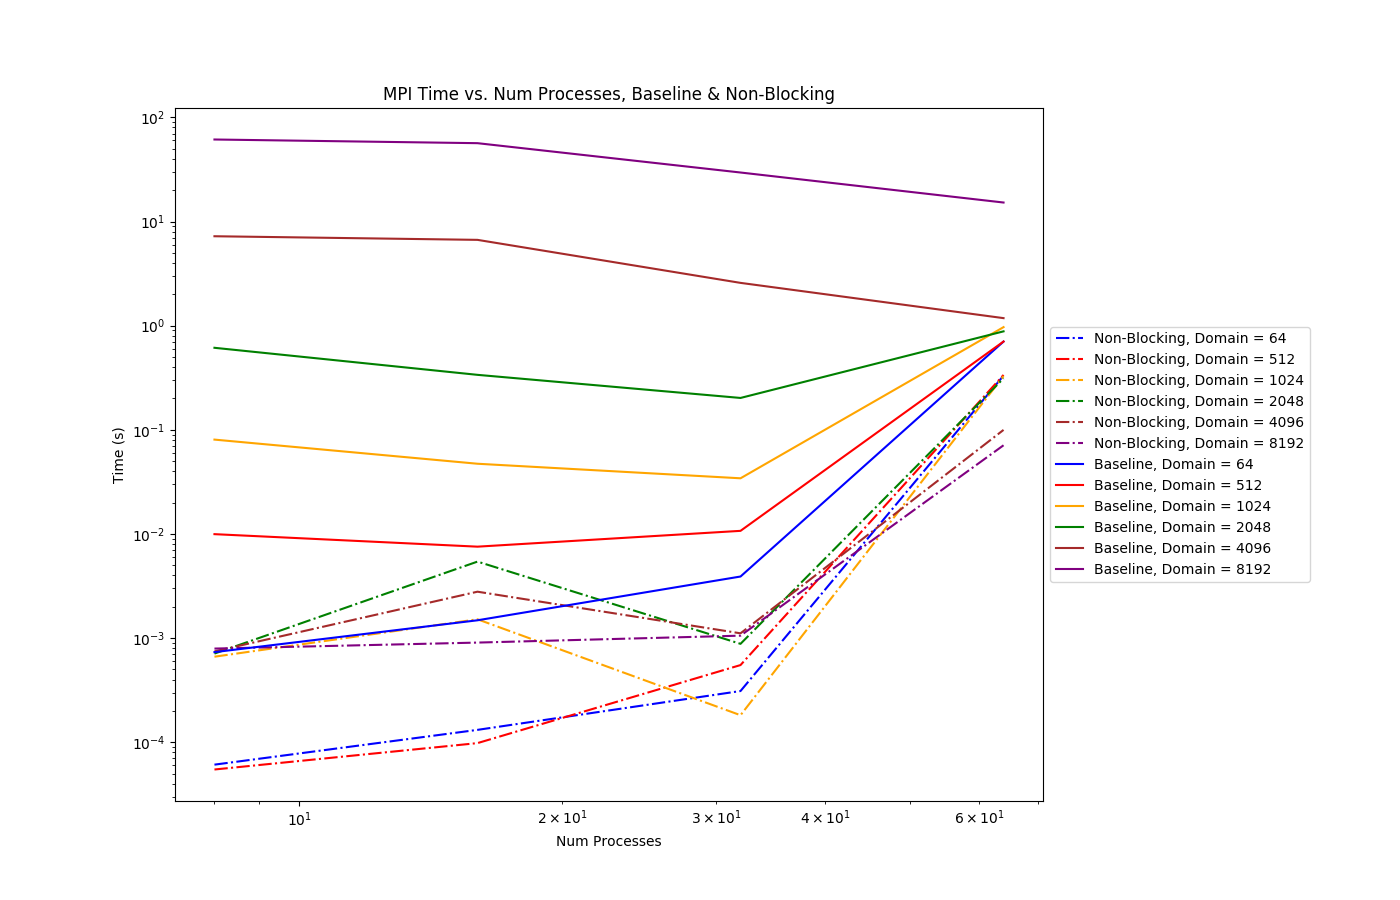
\includegraphics[width=.8\linewidth]{MPI_p2p/mpi_multdomain_haswell_nb_baseline.png} & 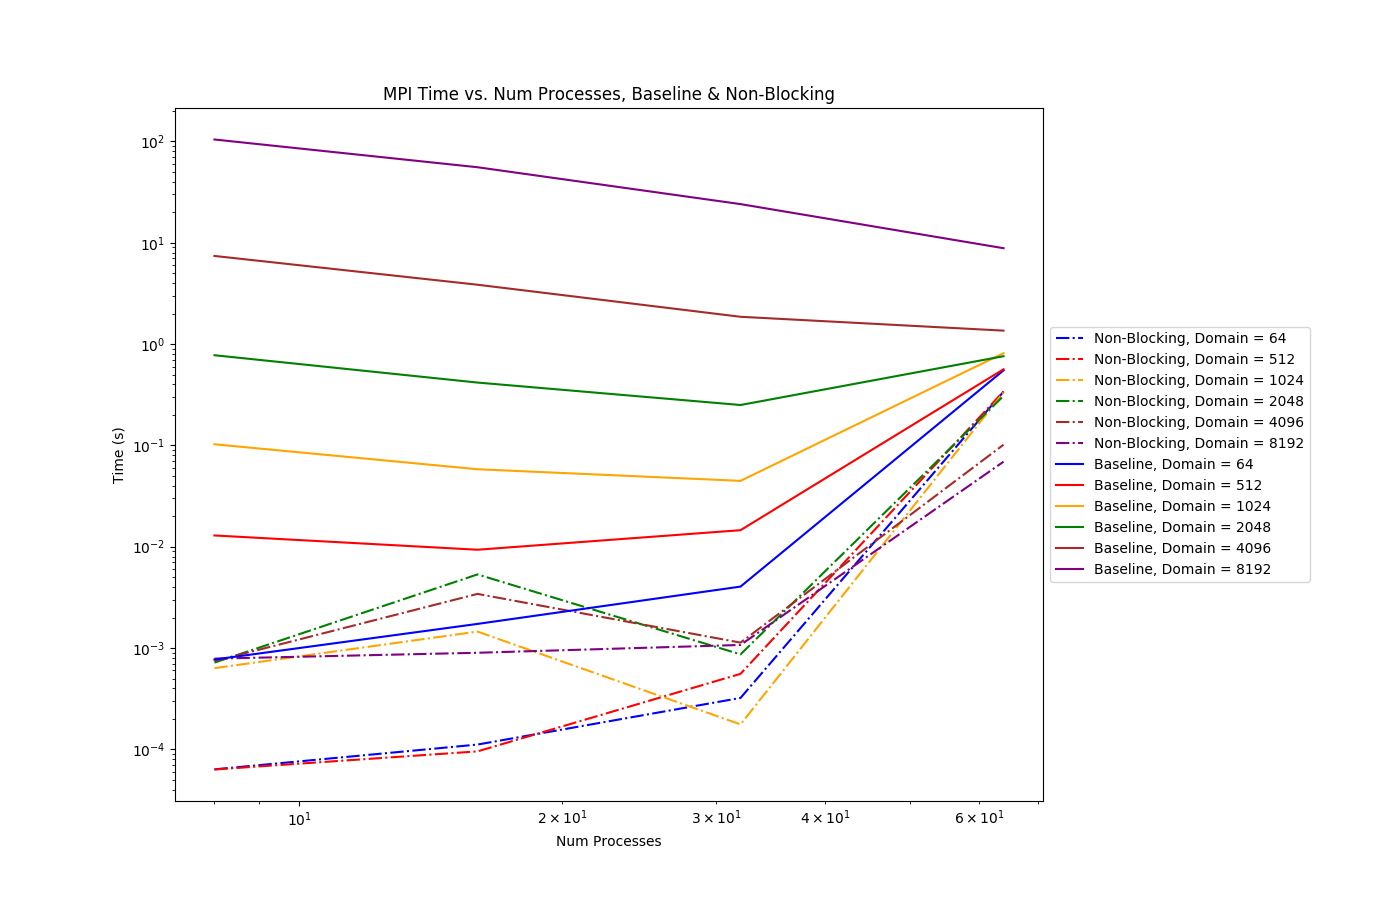
\includegraphics[width=.8\linewidth]{MPI_p2p/mpi_multdomain_sandy_nb_baseline.png} \\
			(a) Haswell &  (b) Sandy Bridge\\[6pt]
		\end{tabular}
		\caption{MPI Time vs. \#Processes., Non-Blocking vs. Baseline}
		\label{fig:mpi_multdomain_nb_baseline}
	\end{figure}
	
		\begin{figure}[h] % h=here, t=top, b=bottom, p=(extra)page, !=force
		\hspace*{-0.25\linewidth}\begin{tabular}{cc}
			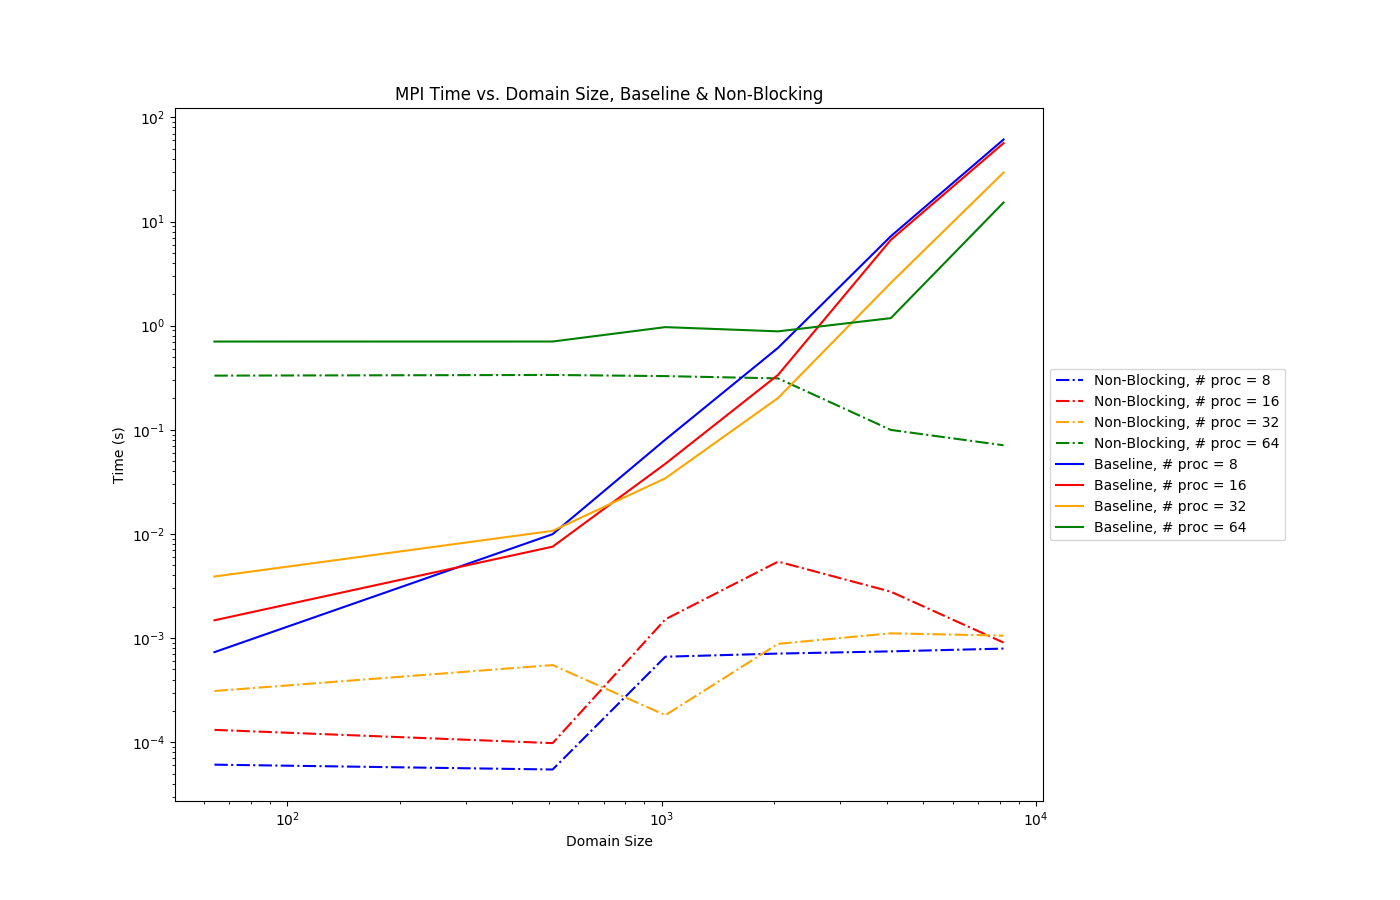
\includegraphics[width=.8\linewidth]{MPI_p2p/mpi_multproc_haswell_nb_baseline.png} & 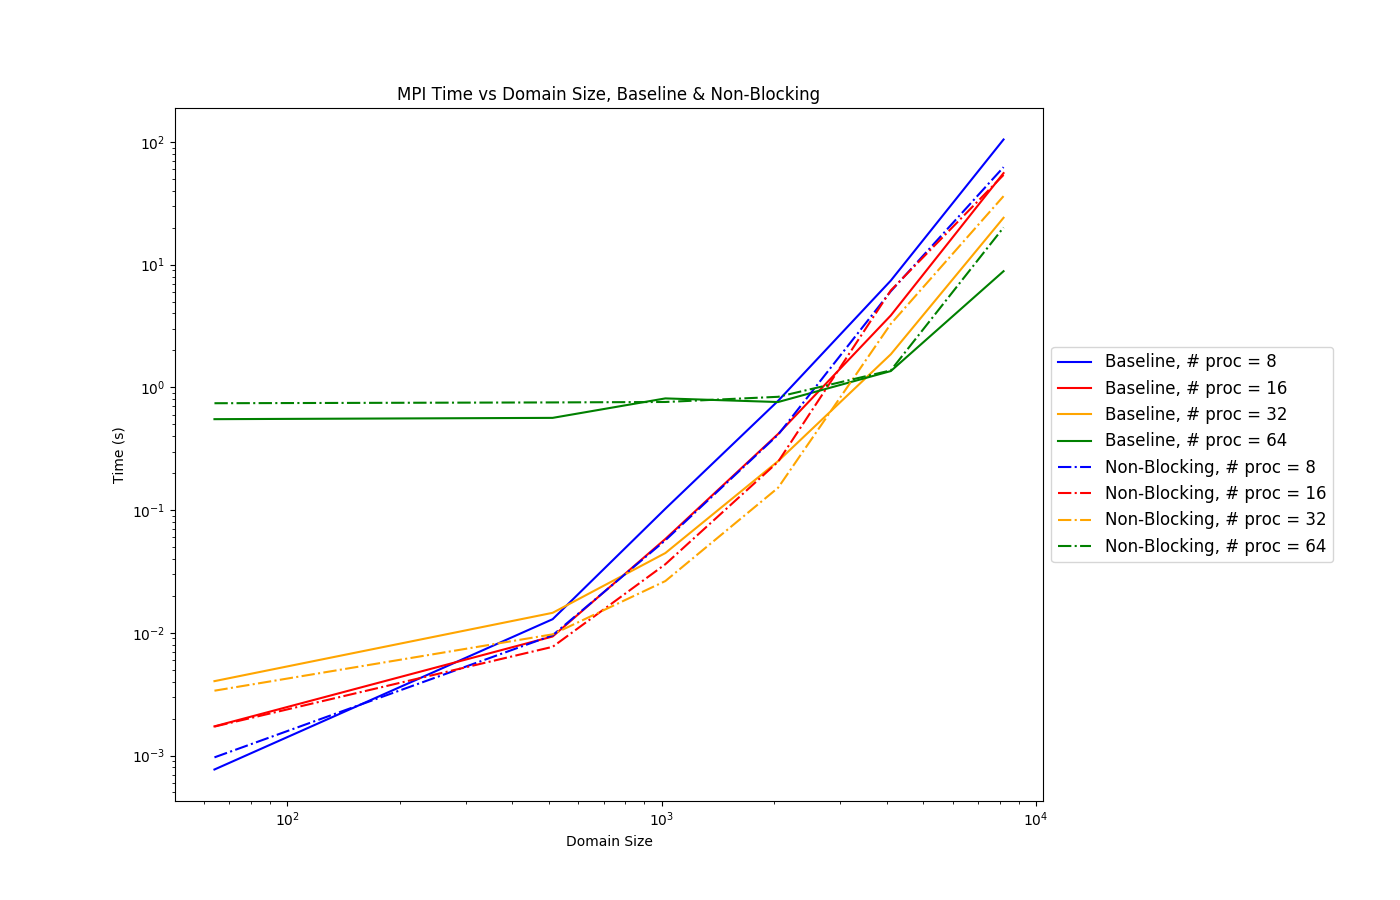
\includegraphics[width=.8\linewidth]{MPI_p2p/mpi_multproc_sandy_nb_baseline.png} \\
			(a) Haswell &  (b) Sandy Bridge\\[6pt]
		\end{tabular}
		\caption{MPI Time vs. Domain Size., Non-Blocking vs. Baseline}
		\label{fig:mpi_multproc_nb_baseline}
	\end{figure}
	
			\begin{figure}[h] % h=here, t=top, b=bottom, p=(extra)page, !=force
		\hspace*{-0.25\linewidth}\begin{tabular}{cc}
			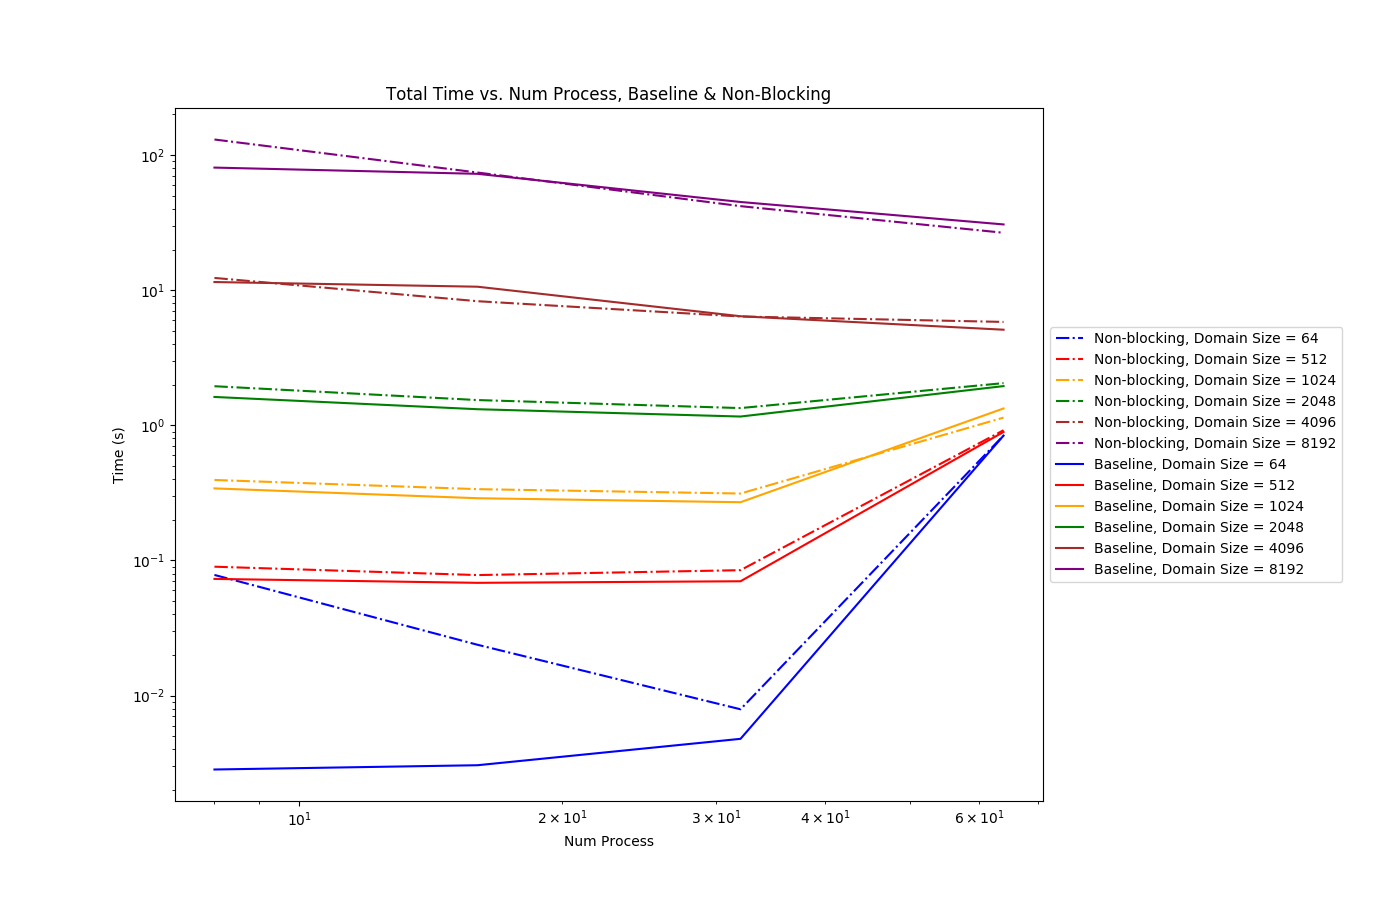
\includegraphics[width=.8\linewidth]{MPI_p2p/total_multdomain_haswell_nb_baseline.png} & 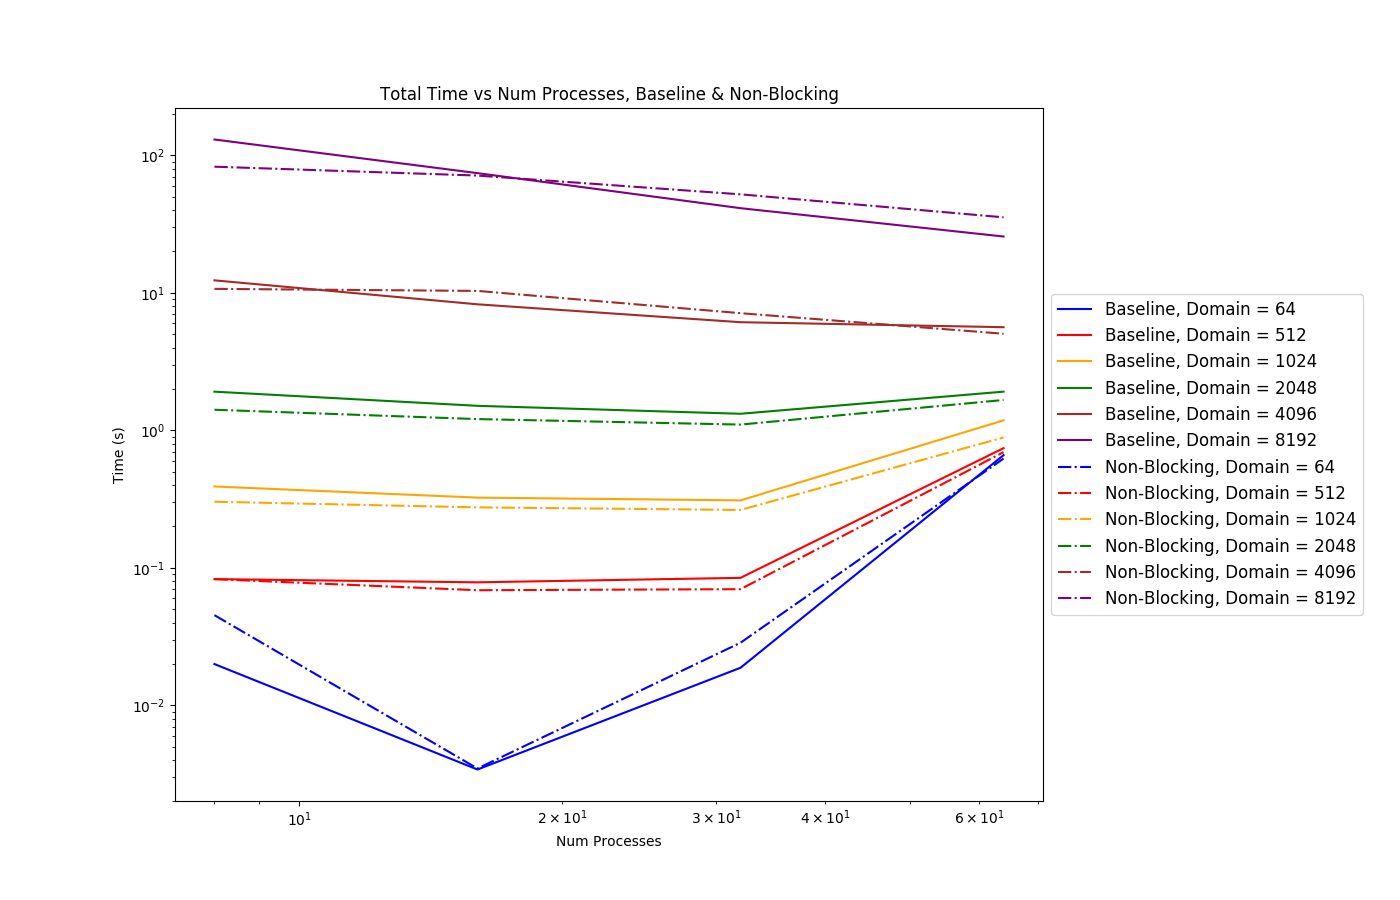
\includegraphics[width=.8\linewidth]{MPI_p2p/total_multdomain_sandy_nb_baseline.png} \\
			(a) Haswell &  (b) Sandy Bridge\\[6pt]
		\end{tabular}
		\caption{Total Time vs. \#Processes., Non-Blocking vs. Baseline}
		\label{fig:total_multdomain_nb_baseline}
	\end{figure}
	
		\begin{figure}[h] % h=here, t=top, b=bottom, p=(extra)page, !=force
		\hspace*{-0.25\linewidth}\begin{tabular}{cc}
			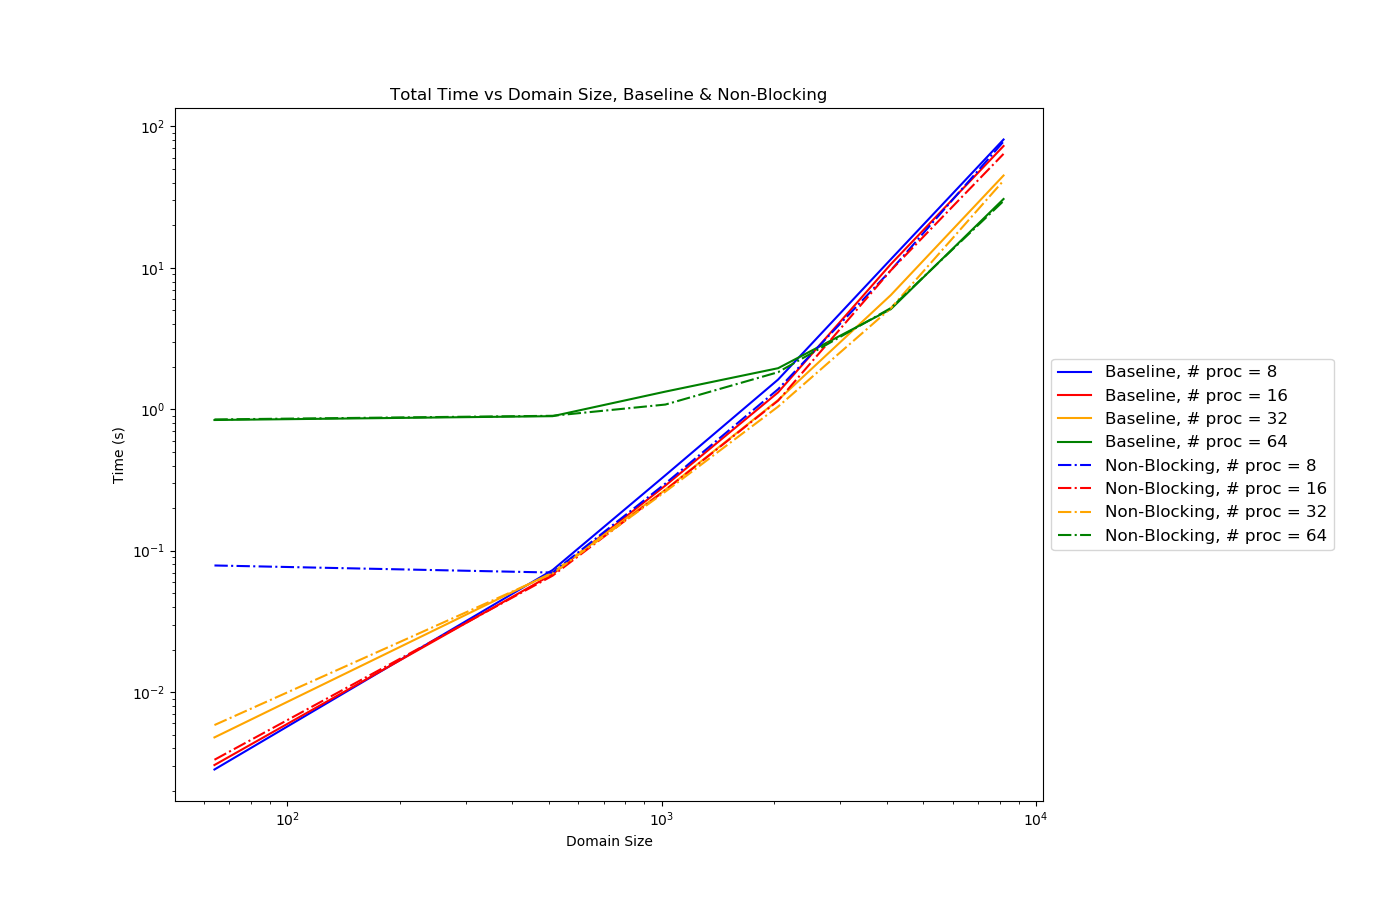
\includegraphics[width=.8\linewidth]{MPI_p2p/total_multproc_haswell_nb_baseline.png} & 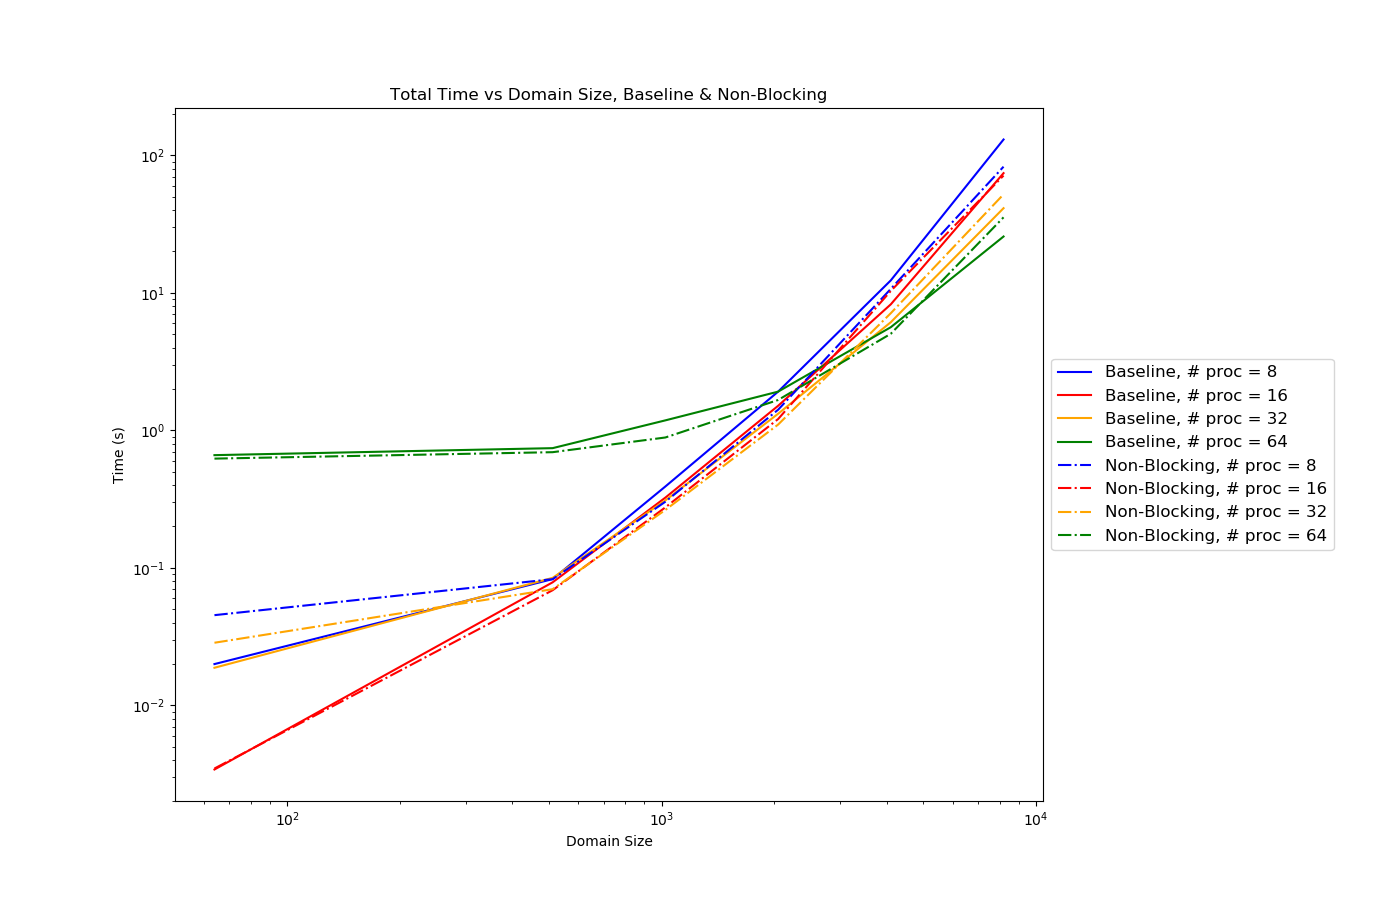
\includegraphics[width=.8\linewidth]{MPI_p2p/total_multproc_sandy_nb_baseline.png} \\
			(a) Haswell &  (b) Sandy Bridge\\[6pt]
		\end{tabular}
		\caption{Total Time vs. Domain Size., Non-Blocking vs. Baseline}
		\label{fig:total_multproc_nb_baseline}
	\end{figure}

\end{enumerate}

% % Figure example
% \begin{figure}[p] % h=here, t=top, b=bottom, p=(extra)page, !=force
%  	\begin{center}
%  		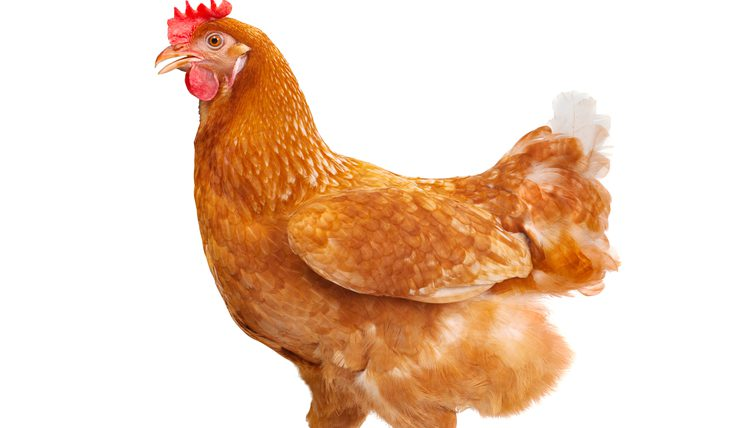
\includegraphics[width=.9\linewidth]{figure.png} % It searches in the Figures/ folder!
%  		\caption{Caption text}
%  		\label{fig:figureLabelName}
%  	\end{center}
% \end{figure}
